A general polynomial equation $p(x,y)$ of degree 2 is given by :
\begin{align}
Ax^2 + Bxy + Cy^2 + Dx + Ey + F = 0
\end{align}
The vector equation of $p(x,y)$ is given by 
\begin{align}
\vec{x^T}\myvec{A & \frac{B}{2} \\ \frac{B}{2} & C}\vec{x} + \myvec{D & E}\vec{x} + F=0\label{sep/2/17eq:1}
\end{align}
As the polynomial we have to find is a quadratic polynomial we have :
\begin{align}
B = 0,
C = 0,
E = 0
\end{align}
If we take $A = 1$ , we have :
\begin{align}
\text{Sum of zeroes} = -D = -3
\implies D = 3\\
\text{Product of zeroes} = F = 2
\end{align}
Substituting the values in \eqref{sep/2/17eq:1}, the required quadratic polynomial is given by :
\begin{align}
\vec{x^T}\myvec{1 & 0 \\ 0 & 0}\vec{x} + \myvec{3 & 0}\vec{x} + 2=0
\end{align}
See Fig.     \ref{sep/2/17Quadratic polynomial with zeroes -1 and -2}
\begin{figure}[!ht]
       \centering
    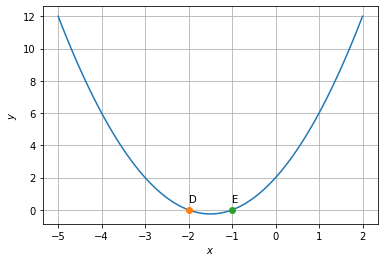
\includegraphics[width=\columnwidth] {solutions/sep/17/Assignment_5_Fig_1.png}
    \caption{Quadratic polynomial with zeroes -1 and -2}
    \label{sep/2/17Quadratic polynomial with zeroes -1 and -2}
\end{figure}

